\chapter{Zugversuche }

\section{Durchführung (ZB)}

Um die Einflüsse der Wärmebehandlungen genauer betrachten zu können, wurden weitere wichtige mechanische Kennwerte wie die Duktilität, Zugfestigkeit und Bruchdehnung von 8 Probendurch einen Zugversuch ermittelt. \\
Um auch den Einfluss von dem Martensitzerfall in der Strategie 1 auf die Duktilität genauer diskutieren zu können, wird auch Probe 4 untersucht. Eine Übersicht über die für den Zugversuch ausgewählten Proben ist in Tabelle \ref{tab:ubersicht} aufgeführt.


\begin{table}[h]
	\centering
	\begin{tabular}{|c|c|}
		\hline 
		Probe & Wärmebehandlung \\ 
		\hline 
		1 & AR1 \\ 
		\hline 
		2 & AR2 \\ 
		\hline 
		3 &  983$^\circ$C/1h/AC + 950$^\circ$C/16min/WQ + 610$^\circ$C/16min/AC \\ 
		\hline 
		4 &  983$^\circ$C/1h/AC + 950$^\circ$C/16min/WQ + 610$^\circ$C/16min/AC \\ 
		\hline 
		5 &  983$^\circ$C/1h/WQ + 610$^\circ$C/30min/AC \\ 
		\hline 
		6 &  983$^\circ$C/1h/WQ + 610$^\circ$C/30min/AC \\ 
		\hline 
		7 &  983$^\circ$C/1h/AC + 950$^\circ$C/16min/WQ \\ 
		\hline 
		8 &  983$^\circ$C/1h/AC + 950$^\circ$C/16min/WQ \\ 
		\hline 
	\end{tabular}
    \caption{Übersicht der gewählten Proben für den Zugversuch}
	\label{tab:ubersicht} 
\end{table}

\section{Ergebnisse (VR)}

Die gesamten Ergebnisse der Zugversuche sind in \ref{tab:zugversuche} zusammengefasst. Man erkennt eine Zugfestigkeitssteigerung bei allen Wärmebehandlungen gegenüber den AR-Proben. Die TS-STDA hat eine Steigerung der Zugfestigkeit von 7,6\% mit Martensitzerfall, 4,3\% ohne Martensitzerfall und die $\alpha_p + \alpha^\prime$-Strategie 1,3\%  gebracht. Die Bruchdehnung ist jedoch bei allen wärmebehandelten Proben unter die geforderten 10\% gefallen. 
Wie in Abbildung \ref{fig:zugkaputt} zu sehen ist, sind alle Proben am Rand des parallelen Fließbereichs der Zugprobe eingeschnürt und gebrochen. Dies hat zur Folge das nicht die gesamte Dehnung der Probe von den Wegaufnehmern aufgenommen wurde und die tatsächliche Dehnung der Proben wahrscheinlich höher ist als gemessen. In den Spannungs-Dehnungs-Diagrammen in den Abb. \ref{fig:vergleich-vor-und-nach-zerfall}--\ref{fig:vergleich-alle-proben} ist eine Hysteresekurve im Bereich von 1\% Dehnung zu sehen. Sie wird automatisch vom Steuerungsprogramm der Zugmaschine durchgeführt, um Abweichungen im elastischen Werkstoffverhalten zwischen Be- und Entlastung aufzunehmen. 


\begin{figure}
	\centering
	\includegraphics[width=0.6\linewidth]{./Bilder/Zugproben_kaputt}
	\caption{links: $\alpha_p + \alpha^\prime$-Probe, mitte und rechts: TS-STDA}
	\label{fig:zugkaputt}
\end{figure}

\begin{figure}
	\centering
	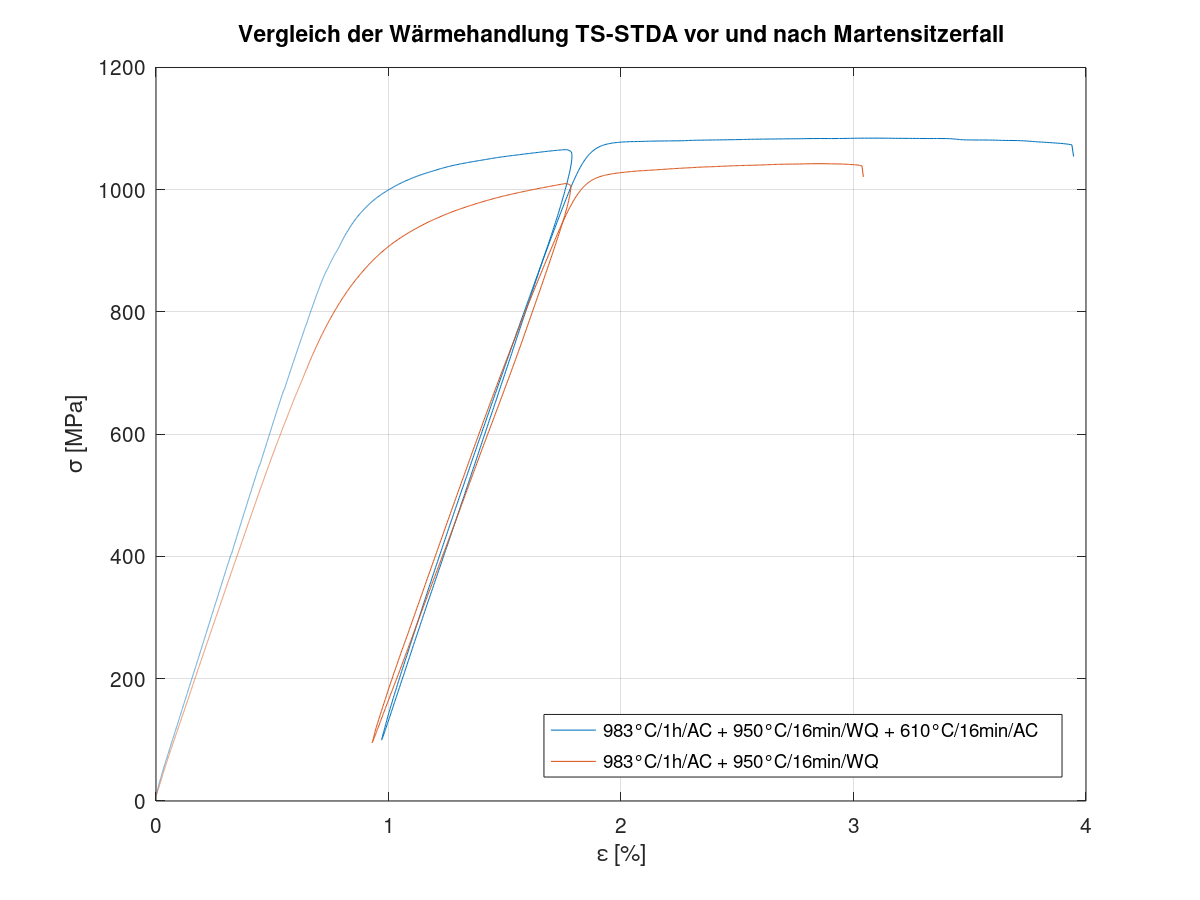
\includegraphics[width=0.7\linewidth]{./Bilder/Vergleich vor und nach Zerfall}
	\caption{Spannungs-Dehnungs-Diagramm für TS-STDA vor und nach dem Martensitzerfall}
	\label{fig:vergleich-vor-und-nach-zerfall}
\end{figure}

\begin{figure}
	\centering
	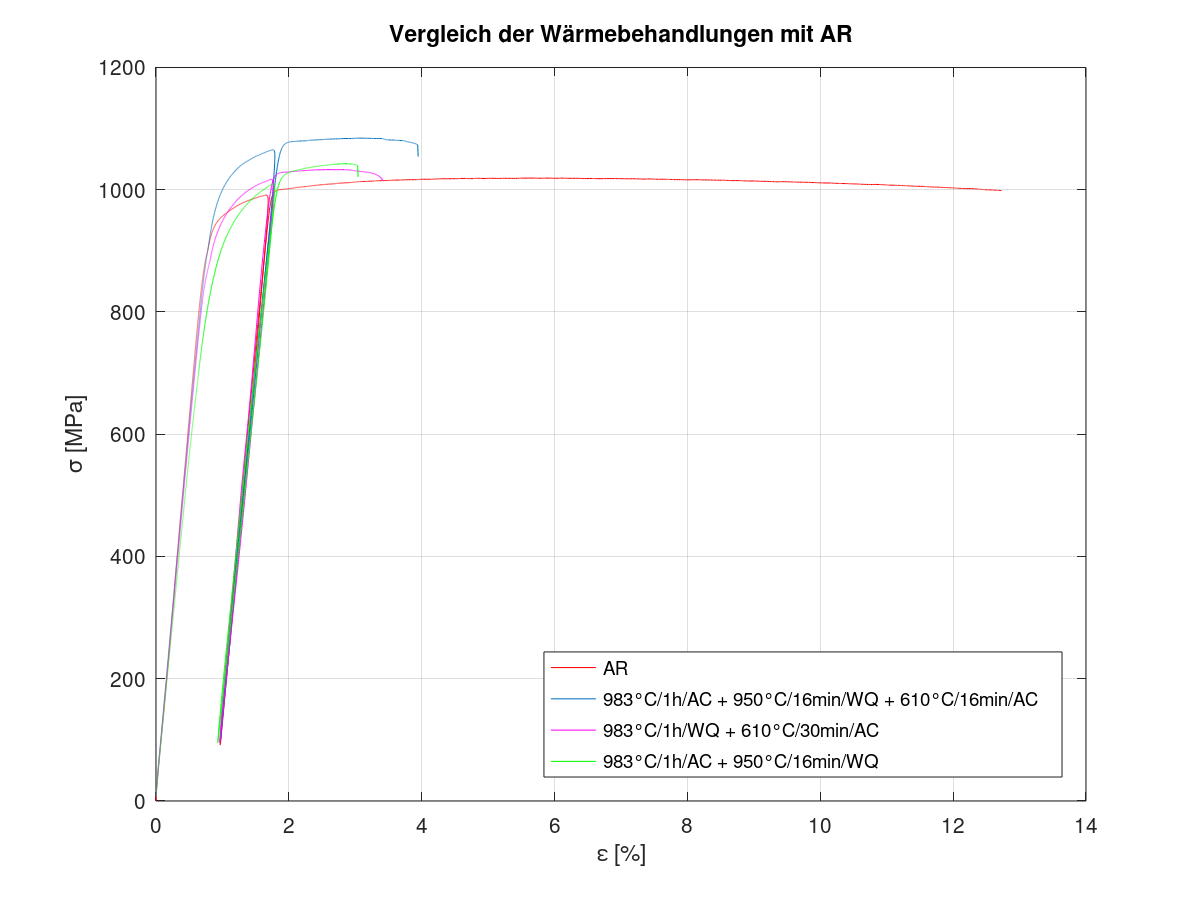
\includegraphics[width=0.7\linewidth]{./Bilder/Vergleich aller Proben}
	\caption{Spannungs-Dehnungs-Diagramm für alle Proben}
	\label{fig:vergleich-alle-proben}
\end{figure}



\begin{table}[h]
	\centering
	\begin{tabular}{|c|c|c|c|c|c|c|c|}
		\hline
		Probe & $d_0$ [mm] & $S_0$ [mm$^2$] & E [GPa] & $R_{p0,2}$ [MPa]& $R_m$ [MPa]& $A_g$ [\%]& $A$ [\%]\\
		\hline
		1 & 5,06 & 20,11 & 128 & 956 & 1019&4,8&17,9 \\
		\hline
		2 &5,04&19,95&122&946&1013&5,1&15,7\\
		\hline
		3 & 5,11&20,51& 122&1015&1085&2,1&3,0\\
		\hline
		4 &5,16& 20,91& 117 & 1007& 1090& 1,7&  1,9 \\
		\hline
		5&5,04 &19,95& 120& 952& 1033& 1,9 &2,5\\
		\hline
		6 &5,02& 19,79& 124& 968& 1023 &1,0 & 2,0\\
		\hline
		7&5,17& 20,99& 113& 925& 1042& 1,9& 2,1\\
		\hline
		8 & 5,12 & 20,59 & 118 & 952 & 1063 & 1,3 & 1,4\\
		\hline
	\end{tabular}
	\caption{Messwerte der Zugversuche bei 23,3$^\circ$ C Raumtemperatur}
	\label{tab:zugversuche}
	
\end{table}

\section{Diskussion der Ergebnisse (ZB)}

Es wurde im Rahmen der Zugversuche festgestellt, dass alle Probenbrüche außerhalb der Messstrecke liegen, das zu einer Ungenauigkeit der gemessenen Bruchdehnungen führt. Es ist daher mit höheren Duktilitätswerten zu rechnen. \\

AR-Proben haben ein globulares Gefüge mit $\alpha$- und transformierte $\beta$-Phase (Abbildung \ref{fig:abbildung-8}). Durch den großen Anteil an $\alpha_p$ konnten sich sehr feine $\alpha$-Lamellen in der kleinen transformierten $\beta$-Phase bilden. Aufgrund dieser feinen Strukturen haben AR-Proben eine relativ hohe Bruchdehnung.

\paragraph{Strategie 1}
Nach dem 2. Schritt (Kapitel \ref{MB1}) hat sich Martensit in der Transformierten $\beta$-Phase des bimodalen Gefüges gebildet. Die feinere Gefügestruktur  durch die dünnen Martensitnadeln und die feinen $\alpha$-Lamellen  haben nur zu einer leichten Festigkeitssteigerung bei Probe 5 und 6 geführt. Die Duktilität hat hingegen stark  abgenommen.
Nach dem 3. Schritt (Kapitel \ref{MZ1}) ist die Zugfestigkeit der Proben 3 und 4 durch die weitere Verfeinerung des Gefüges weiter gestiegen. Im Gegensatz zu Proben 5 und 6 , hat die Duktilität bei Probe 3 leicht zugenommen. Das ist  darauf zurückzuführen, dass sich  $\alpha$ und  $\beta$ Phasen, die eine höhere Duktilität im Vergleich zu Martensit besitzen, durch den partiellen Martensitzerfall gebildet haben.


\paragraph{Strategie 2}
%Proben 7 und 8 zeigen gegenüber die anderen Proben eine relativ hohe Zugfestigkeit.  Dies ist durch die feinen Martensitplatten, die ca. 80\% der Probenoberfläche repräsentieren, zu erklären.
%Mit einer längeren Anlasszeit bzw. einer höheren Temperatur im 
%2. Schritt ist eine höere Duktilität durch die Einstellung eines gröberen Gefüges  zu erwarten.
%\newline

Es ist auch zu erkennen, dass es bei allen wärmebehandelten Proben zu einer Zugfestigkeitssteigerung und einer signifikanten Duktilitätsabnahme gekommen ist.\\
Die Proben 7 und 8 haben durch das Duplex-Glühen neben Martensit und kleinen $\alpha_p$-Körnern feine $\alpha$-Lamellen. Außerdem haben die Proben 5--8 im Vergleich zu den AR-Proben durch die Bildung von  dünnen Martensitplatten feinere Gefügestrukturen. Das führte anscheinend bei diesen Proben zu der Festigkeitszunahme. Das erklärt auch, dass Martensit, der nur eine beschränkte Duktiliät besitzt \cite{Lutjering.2007}, zu der niedrigen Duktilität dieser Proben geführt hat.\\
Des Weiteren hat die Probe 3 eine höhere Duktilität und Festigkeit gegenüber den Proben 7 und 8. Das kann durch den partiellen Martensit-Zerfall bzw. die Teiltransformation von $\alpha'$ in $\alpha$- und $\beta$-Phasen im letzten Schritt der Strategie 1 erklärt werden. Die Verfeinerung des Gefüges durch eine partielle Dekomposition der Martensitnadeln führt einerseits zu einer Steigerung der  Zugfestigkeit  und gleichzeitig zu einer Zunahme der Duktilität. 
Das heißt, dass eine weitere Dekomposition der Martensitstrukturen bei beiden Strategien zu einer Verbesserung der Bruchdehnung führen könnte. Dabei soll sich eine gröbere Gefügestruktur durch die Transformation von Martensit vollständig in $\alpha$- und $\beta$-Körner bilden. Dies ist möglich, wenn Proben beim letzten Anlassen für längere Zeit bzw. bei höheren Temperaturen geglüht werden.



\begin{table}[h]
	\centering
	\begin{tabular}{|c|c|}
		\hline 
		Strategie & Wärmebehandlung \\ 
		\hline 
		1 & 983$^\circ$C/1h/AC + 950$^\circ$C/16min/WQ + 610$^\circ$C/1h/AC\\ 
		\hline 
		2 &  983$^\circ$C/1h/WQ + 800$^\circ$C/2h/AC \\ 
		\hline 
	\end{tabular} 
	\caption{}
	\label{wBZ}
	
	
\end{table}

Durch beide Strategien konnte immerhin  eine Verfestigung von Ti-6242 erreicht werden. Die Dehngrenze hat dabei  die 10\% unterschritten. Strategie 1 hat aber im Vergleich zu Strategie 2 signifikante Schwankungen gezeigt(Siehe Tabelle \ref{tab:zugversuche}). Das ist vor allem durch die kurzen Anlasszeiten und der starken Einfluß der Glühtemperatur auf die Gefügestruktur bedingt. \\
Wird Strategie 2  nach den gewünschten Gefügeeigenschaften entwickelt und angepasst, so ist sie auf jeden Fall kürzer als die häufig verwendete Strategie 2.













